\documentclass{standalone}

\usepackage{color}
\usepackage{tikz}
\usetikzlibrary{positioning}


% \definecolor{myred}{RGB}{175,53,71}
% \definecolor{myblue}{RGB}{0,116,188}


\newcommand{\freeParticle}[1]{\ensuremath{v_{#1}}}
\newcommand{\fixedParticle}[1]{\ensuremath{f_{#1}}}
\newcommand{\spring}[1]{\ensuremath{k_{#1}}}

\newcommand\numFreeRowsCols{3}
\newcommand\gridSpacing{1.6}

\tikzset{
		edgeStyle/.style = {line width = 1.3pt},
		fixed/.style = 		 {anchor=base,fill,circle,inner sep=1.5pt},
		free/.style =	     {circle,draw, inner sep = 1pt},
    spring/.style =    {fill=white,circle,inner sep = 0.1pt, anchor=center, midway},
		node distance=2.3cm
}

\newcommand{\drawFixedParticles}[1]{
      % Draw upper row of fixed nodes
    {
      \newcommand\y{#1}  
      \pgfmathtruncatemacro{\yi}{\y - 1}
      \foreach \x in {0,...,\numRowsCols}
      {
        \pgfmathtruncatemacro{\label}{\x}
        \pgfmathtruncatemacro{\springlabel}{\x}
        \node [fixed] (\x\y) [label=above:{\fixedParticle{\label}}] at (\gridSpacing*\x,\gridSpacing*\y) {};
        \draw (\x\y)--(\x\yi) node[spring] {\spring{\springlabel}};
      }
    }

    % Draw lower row of fixed nodes
    {
      \newcommand\y{-1}  
      \pgfmathtruncatemacro{\yi}{\y + 1}
      \foreach \x in {0,...,\numRowsCols}
      {
        \pgfmathtruncatemacro{\label}{#1 * 3 + \x}
        \pgfmathtruncatemacro{\springlabel}{\x + #1 * (#1 - 1 - \y) + (#1 + 1) * (#1 - 1 - \y)}
        \node [fixed] (\x\y) [label=below:{\fixedParticle{\label}}] at (\gridSpacing*\x,\gridSpacing*\y) {}; 
        \draw (\x\y)--(\x\yi) node[spring] {\spring{\springlabel}};
      } 
    }

    % Draw left column of fixed nodes
    {
      \newcommand\x{-1}  
      \pgfmathtruncatemacro{\xi}{\x + 1}
      \foreach \y in {0,...,\numRowsCols}
      {
        \pgfmathtruncatemacro{\label}{(2 * #1 - 1) - \y}
        \pgfmathtruncatemacro{\springlabel}{#1 + (#1 - \y - 1) * ((2 * #1) + 1)}        
        \node [fixed] (\x\y) [label=left:{\fixedParticle{\label}}] at (\gridSpacing*\x,\gridSpacing*\y) {}; 
        \draw (\x\y)--(\xi\y) node[spring] {\spring{\springlabel}};
      } 
    }

    %Draw right column of fixed nodes
    {
      \newcommand\x{#1}  
      \pgfmathtruncatemacro{\xi}{\x - 1}
      \foreach \y in {0,...,\numRowsCols}
      {
        \pgfmathtruncatemacro{\label}{(3 * #1 - 1) - \y}
        \pgfmathtruncatemacro{\springlabel}{2 * #1 + (#1 - \y - 1) * ((2 * #1) + 1)}
        \node [fixed] (\x\y) [label=right:{\fixedParticle{\label}}] at (\gridSpacing*\x,\gridSpacing*\y) {}; 
        \draw (\x\y)--(\xi\y) node[spring] {\spring{\springlabel}};
      } 
    }
}

\begin{document}
	
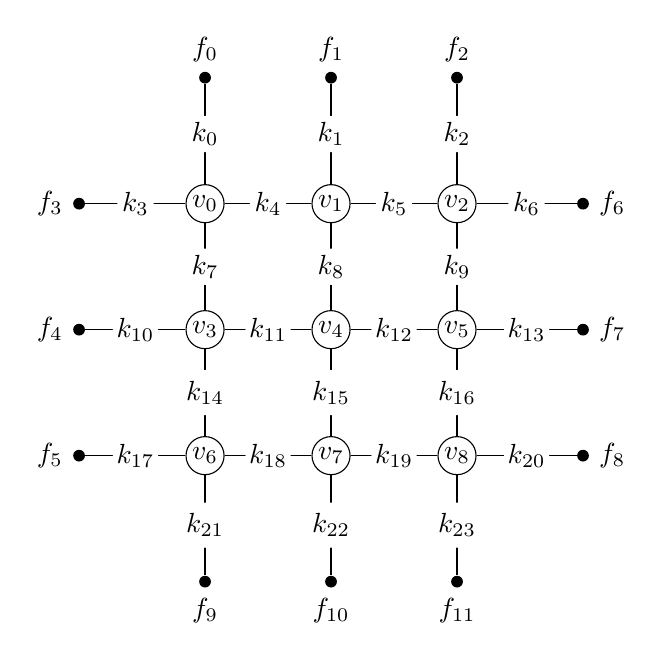
\begin{tikzpicture}
  {
    \pgfmathtruncatemacro{\numRowsCols}{\numFreeRowsCols - 1}
    \pgfmathtruncatemacro{\numRowsColsMinusOne}{\numRowsCols - 1}

    % Draw free particles on grid
    \foreach \x in {0,...,\numRowsCols}
      \foreach \y in {0,...,\numRowsCols} 
         {\pgfmathtruncatemacro{\label}{\x - 3 *  \y + 7 - 1}
         \node [free]  (\x\y) at (\gridSpacing*\x,\gridSpacing*\y) {\freeParticle{\label}};} 

    % Draw edges between free particles in grid
    \foreach \x in {0,...,\numRowsCols}
      \foreach \y [count=\yi] in {0,...,\numRowsColsMinusOne}  {
          % Vertical springs
          \pgfmathtruncatemacro{\label}{\x + \numFreeRowsCols * (\numFreeRowsCols - 1 - \y) + (\numFreeRowsCols + 1) * (\numFreeRowsCols - 1 - \y)}{
            \draw (\x\y)--(\x\yi) node[spring] {\spring{\label}};
          }

          % Horizontal springs
          \pgfmathtruncatemacro{\label}{\y + (\numFreeRowsCols - 1) * (\numFreeRowsCols - 1 - \x) + (\numFreeRowsCols - \x) * (\numFreeRowsCols + 2) - 1}{
            \draw (\y\x)--(\yi\x) node[spring] {\spring{\label}};
          }
          
      }

      \drawFixedParticles{\numFreeRowsCols}      
  }

  

\end{tikzpicture}	

\end{document}
